As not all of the dataset samples were of the same quality it was important to first manually filter the dataset to remove the bad imaging samples. Even with the normal conditions many of the images contain a lot of background. This creates a background vs. foreground class imbalance (see Figure \ref{fig:bad-smaples}a). Overexposure is also a typical problem that creates samples of a too high intensity and with details inside the nucleus missing (see Figure \ref{fig:bad-smaples}b, c). Lastly, underexposure is just as problematic as overexposure (see Figure \ref{fig:bad-smaples}d).

\begin{figure}[H]
	\begin{center}
		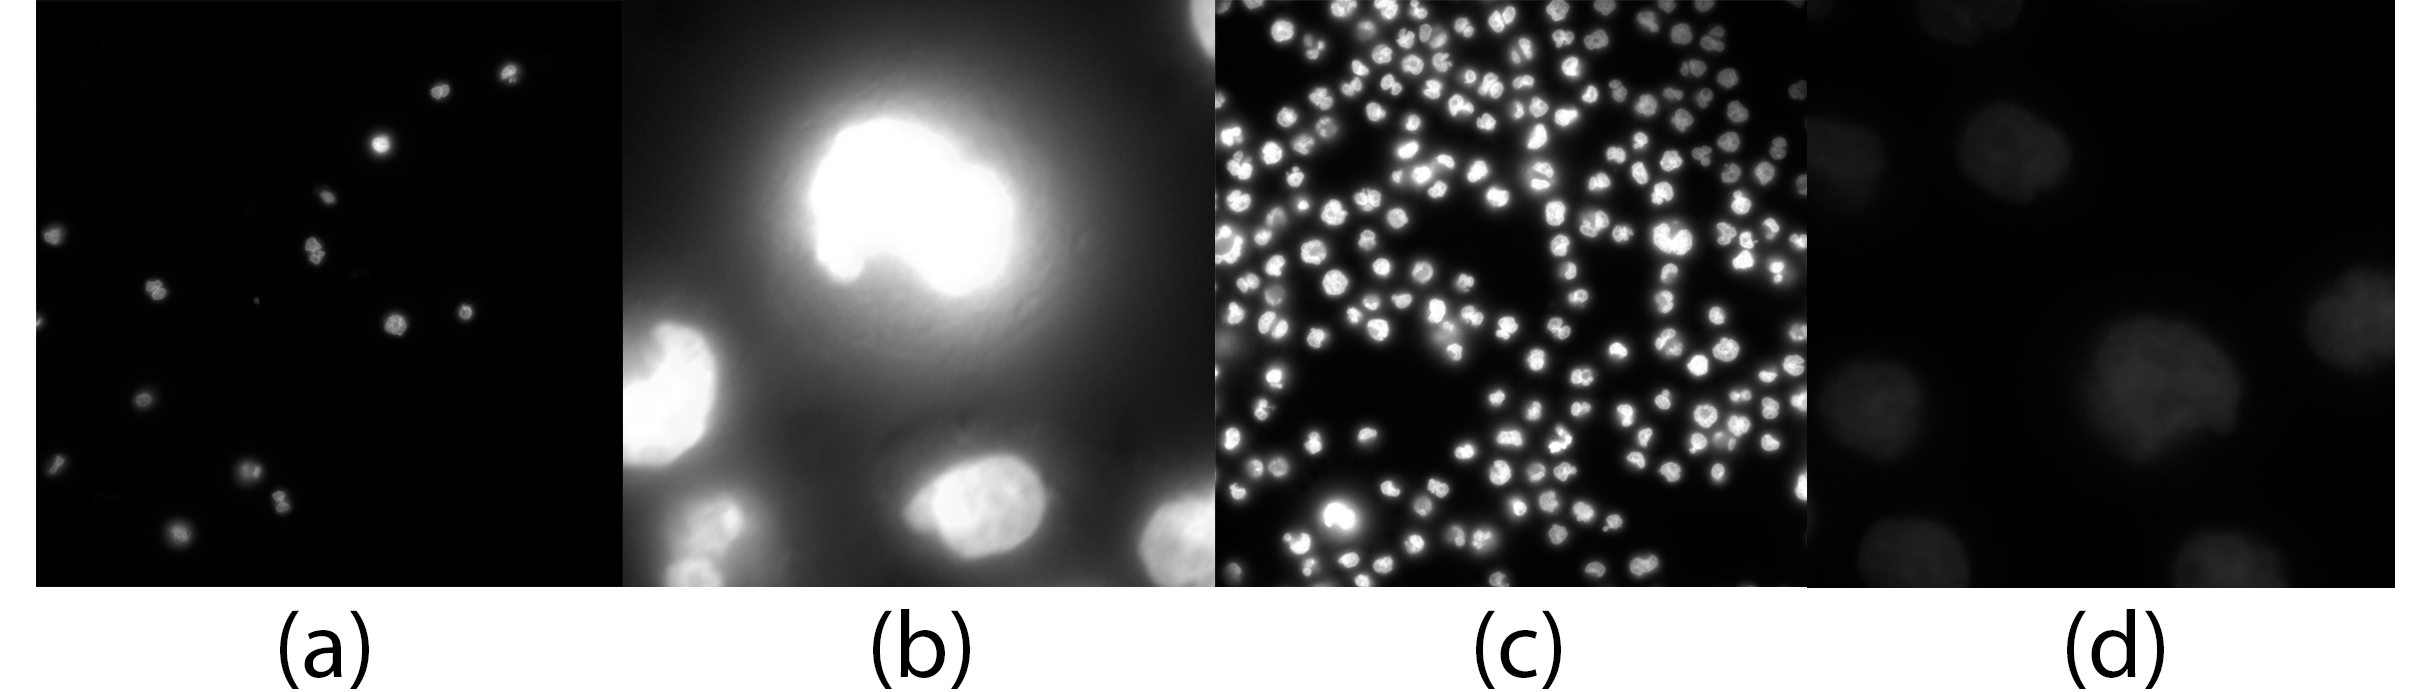
\includegraphics[width=0.7\linewidth]{bilder/nuclei/filter-out.png}
		\caption[Nuclei fluorescence samples to be filtered out]%
		{Nuclei fluorescence samples to be filtered out. (a) --- too few cells in the image result in many fully black crops; (b) --- overexposure; (c) --- overexposure, lack of details; (d) --- underexposure.}\label{fig:bad-smaples}
	\end{center}
\end{figure}

Once the images have been filtered out, they were normalized to have the values between 0 and 1.
